In Chapter 4~\ref{ch:ecf}, we briefly introduced ECF Modules, describing them as an encapsulated set of functionality operating on a specific programming environment feature.
Since this point, we have treated them as helpful back boxes without profoundly understanding their concrete design.

In this chapter, we will analyze each ECF Module available in the EasyFly extension in detail, describing the purpose, main functionality, and implementation details for each. 
First, We will give an overview of the concept behind the ECF Modules, understanding the motivations and principles that make these modules the most essential part of the EasyFly programming environment.
Then, we will enter in the detail of each ECF Module implemented, providing the specific utility and use cases.

\section{ECF Modules Overview}\label{sec:modules_overview}
For a programming environment like EasyFly that is meant to be used for HDI research, the system's modularity is a key feature that cannot be missed.
In fact, a modular system allows the configuration to adapt to any possible change in the surrounding environment or the application's requirements.

As we have seen in the final example of the previous chapter (see Listing~\ref{example_coordination}), the resulting code is still full of repetitive operations that make the code less clear and prone to errors.
For this reason, our EasyFly programming environment is still missing a lot of automatic processes that can help reduce developers' effort and increase usability. 

If we look in detail at the process adopted to solve the previous chapter's example, we can identify four main steps:
\begin{enumerate}
    \item Define the state of the application and \( \langle Event, Condition, Action \rangle \) tuples
    \item Setup the Coordination Framework to handle that state
    \item Setup the Logging Manager to update correctly that state
    \item Define how and when reacting to state changes
\end{enumerate}

Given the fact that almost any drone application can be modeled using\\
\( \langle Event, Condition, Action \rangle \) tuples, we can undoubtedly apply the above solution methodology for all such applications.
Moreover, we can say that the process's most challenging and application-related part is the first step; the other parts are straightforward.

Since the possible states of an application depend mainly on the basic information that the platform provides, like telemetry data, we can automatize the setup process (points 2 and 3) for the basic information.
For example, since most of the applications will use the estimated position of the Crazyflie, we can create a \textit{standard state} containing position-estimated information and maintain it updated using the Coordination Framework.

In this way, every developer who needs estimated position information can access this standard state and use the information as required.

The ECF Modules are the software components that implement the automatic process of updating standard states. Moreover, they add the modularity feature to our programming environment.

Sometimes, the simple raw information is useless for a developer; therefore, the ECF Modules usually contain a set of functionality that allows the processing of the information cleverly. 


\section{State Estimate Module}\label{sec:module_state_estimate}
Regardless of the purpose, a crucial aspect of operating a drone is having a deep understanding of the drone's position, velocity, and acceleration. 
These parameters are vital for ensuring the drone's stability and safe navigation. 
Accurate knowledge of the drone's position and speed enables its operator to control its movements and avoid obstacles or hazards in its path. 
Furthermore, understanding acceleration is crucial in achieving precision and accurate control of the drone's movements.
State estimate accuracy depends on how much information the control loop can use. 
In particular, the decks that contribute more to the estimation process are the Lighthouse positioning Deck and the Flow Deck V2. 

As the name suggests, the State Estimate Module is an ECF Module that manages the estimated variables of the Crazyflie 2.1.
The role of this module is to keep the information relative to the estimated variables inside the Coordination Framework updated.
In this way, a developer that needs this information finds them already in the Coordination Framework instead of losing time setting up the logging on their own.

The full state of the State Estimate ECF Module is detailed in Table~\ref{table:estimate_module_state}

\begin{table}[tb]
    \centering
    \begin{tabular}{*{2}{|c}|}
    \hline
    \rowcolor{bluepoli!40}
    \textbf{Variable} & \textbf{Description} \\
    \hline \hline
    x & Position on the x-axis from the origin \\
    \hline
    y & Position on the y-axis from the origin \\
    \hline
    z & Position on the z-axis from the origin \\
    \hline\hline
    vx & Velocity on the x-axis \\
    \hline
    vy & Velocity on the y-axis \\
    \hline
    vz & Velocity on the z-axis \\
    \hline\hline
    ax & Acceleration on the x-axis \\
    \hline
    ay & Acceleration on the y-axis \\
    \hline
    az & Acceleration on the z-axis \\
    \hline\hline
    roll & Roll in rad \\
    \hline
    pitch & Pitch in rad \\
    \hline
    yaw & Yaw in rad \\
    \hline\hline
    rateRoll & Roll rate in rad/s \\
    \hline
    ratePitch & Pitch rate in rad/s \\
    \hline
    rateYaw & Yaw rate in rad/s \\
    \hline
    \end{tabular}
    \\[10pt]
    \caption{ECF State Estimate Module's state.}\label{table:estimate_module_state}
\end{table}

Because the control loop onboard the Crazyflie 2.1 runs at 500Hz, a new estimation is computed every two milliseconds; these variables can rapidly change over time. 
We need to update the state as frequently as possible to ensure that the information provided is accurate and precise. 
For this reason, we selected the lowest possible sampling period for the Communication Framework, which is 10 milliseconds.

In this ECF Module, the utility functions allow the user to record the state variable and, at the end of the flight, plot the recorded data.
As with any other telemetry data, it is usually vital for a user to have the possibility to analyze that information after the flight, especially in the development phase of the application.
For this reason, the utility functions that we implemented will allow a user to analyze and compare data from multiple application runs.

\section{Battery Module}\label{sec:module_battery}

When dealing with drones, battery management is an important factor that must always be considered. 
Usually, due to its weight, the battery has minimal capacity, especially on drones with small dimensions.

An application can be perfectly developed, but it can easily fail if it does not consider the limitation of resources like the battery.
To help the developer with this task, we created another ECF Module that manages battery-related information and keeps them updated.

Given this, the full state of the Battery ECF Module is shown in Table~\ref{table:battery_module_state}


\begin{table}[tb]
    \centering
    \begin{tabular}{*{2}{|c}|}
    \hline
    \rowcolor{bluepoli!40}
    \textbf{Variable} & \textbf{Description} \\
    \hline \hline
    pm\_state & Battery power management state \\
    \hline
    voltage & Battery voltage in V \\
    \hline
    battery\_level & Estimated battery level in percentage \\
    \hline
    \end{tabular}
    \\[10pt]
    \caption{ECF Battery Module's state.}\label{table:battery_module_state}
\end{table}

The first variable of the state, \textit{pm\_state}, represents the state in which the power management of the drone is in.
The state can be one of the following:
\begin{itemize}
    \item Battery -- The drone is on and using its battery.
    \item Charging -- The drone is plugged into the power supply.
    \item Charged -- The drone has completed the recharge, and its battery is fully charged.
    \item Low Power -- The drone needs to be recharged.
\end{itemize}

With the other two properties of the state, \textit{voltage} and \textit{battery\_level}, the developer can determine with high precision the recharging phase.

Since battery management strictly depends on the application to be developed, it is hard to find an implementation that satisfies all the possible usage.
For this reason, the module is responsible only for keeping the information in the state consistent and updated.

\section{Multiranger Module}\label{sec:module_multiranger}

The Multiranger deck is an accessory board for the Crazyflie 2.1. 
The deck is designed to provide the drone with range-sensing capabilities, allowing it to detect objects and obstacles in its environment.

The Multiranger deck features four integrated ultrasonic sensors, which can be used to measure distances in a range of up to 4 meters. 
These sensors emit high-frequency sound waves that bounce off of nearby objects and return to the deck, allowing the deck to calculate the distance to the objects based on the time it takes for the sound waves to return.
Multiranger deck is a powerful tool for adding range sensing capabilities to the Crazyflie 2.1, enabling it to perform a range of applications such as mapping, autonomous navigation, and obstacle avoidance.

As with any other ECF Module, the Multiranger Module also has a state it manages. 
Table~\ref{table:multiranger_module_state} shows that the state is composed of the five range measurements, one for each direction it supports.


\begin{table}[tb]
    \centering
    \begin{tabular}{*{2}{|c}|}
    \hline
    \rowcolor{bluepoli!40}
    \textbf{Variable} & \textbf{Description} \\
    \hline \hline
    front & Distance from the nearest obstacle on the front (up to 4m) \\
    \hline
    back & Distance from the nearest obstacle on the back (up to 4m)\\
    \hline
    right & Distance from the nearest obstacle on the right (up to 4m) \\
    \hline
    left & Distance from the nearest obstacle on the left (up to 4m) \\
    \hline
    up & Distance from the nearest obstacle above (up to 4m) \\
    \hline
    \end{tabular}
    \\[10pt]
    \caption{ECF Multiranger Module's state.}\label{table:multiranger_module_state}
\end{table}

Given the wide range of applications the Multiranger deck fits, we decided to implement a simple implementation of two use cases of this deck directly inside the module:
\begin{itemize}
    \item Object Tracking 
    \item Obstacle Avoidance
\end{itemize}

With the Object Tracking behavior, the drone searches for an object to track when it starts. 
As soon it detects an object inside a configurable range, that object becomes the guide to follow. 
The drone with this behavior will try to follow whenever the tracked object moves in space. 

The velocity needs to change depending on the distance from the object. 
If the object is on the perimeter of the activation range, we need to move fast towards it, trying not to lose the tracking. 
On the other hand, when the object is closer to the safe range, the velocity can be slowed since the object is closer to the drone.
The drone uses the safe range to never hit the tracked object.

In summary, as we can see in Figure~\ref{fig:multiranger_tracking}, the drone with an Object Tracking behavior has two ranges:
The first range, which is the activation range, is used to determine what the tracked object is.
The second range, the safety range, is used to prevent collision with the tracked object when it stands at a fixed point.

\sidecaptionvpos{figure}{c}
\begin{SCfigure}[\sidecaptionrelwidth][tb]
    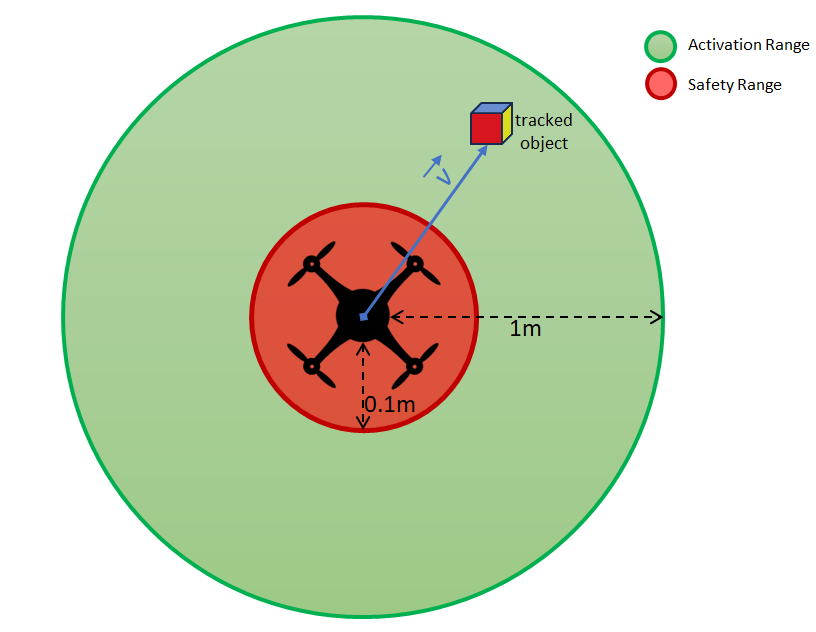
\includegraphics[width=0.5\textwidth]{modules/multiranger}
    \caption{Multiranger Object Tracking behavior.}\label{fig:multiranger_tracking}
\end{SCfigure}

The Obstacle Avoidance behavior is the opposite behavior with respect to object tracking. 
In this case, the activation range is used to determine an obstacle to fly away from.

When an obstacle is detected on the perimeter of the activation range, the drone will slowly start moving in the opposite direction. 
If the obstacle is dynamic and gets closer, the drone will increase its speed to try to escape from the obstacle.

In this behavior, the safety limit is used for landing the drone. 
If the obstacle gets too close, the only thing the drone can do to avoid the collision is landing.

\section{Height Module}\label{sec:module_height}

As we have seen in Section~\ref{deck:flow}, both the Flow deck V2 and the ZRanger deck V2 mount a sensor that allows the drone to measure its height from the ground.
Like the sensors equipped by the Multiranger deck, this sensor enables the height measurement of up to 4 meters, with very high precision.
We designed the height module to manage the information provided by this sensor to simplify height-related tasks in drone applications.

The height module is an ECF module that manages the drone's height. It holds a simple state that consists of a single variable: the height (Shown in Table~\ref{table:height_module_state} ).
\begin{table}[tb]
    \centering
    \begin{tabular}{*{2}{|c}|}
    \hline
    \rowcolor{bluepoli!40}
    \textbf{Variable} & \textbf{Description} \\
    \hline \hline
    height & Height from the ground (up to 4m) \\
    \hline
    \end{tabular}
    \\[10pt]
    \caption{ECF Height Module's state.}\label{table:height_module_state}
\end{table}

When either the Flow deck V2 or the ZRanger deck V2 are attached to the drone, the control loop will use the information provided by the sensor to estimate the internal state of the drone.

At first glance, this contribution seems valuable and harmless; in reality, this is true only when the ground surface is almost flat.
When the ground surface is uneven, the measurement of the height sensor will act as a noise to the state estimation process, especially if the ground presents a stepped surface.

To better understand the uneven floor problem, let us consider the example shown in Figure~\ref{fig:uneven_floor}.

\begin{figure}[tb]
    \centering
    \subfloat[Flat ground\label{fig:uneven_a}]{
        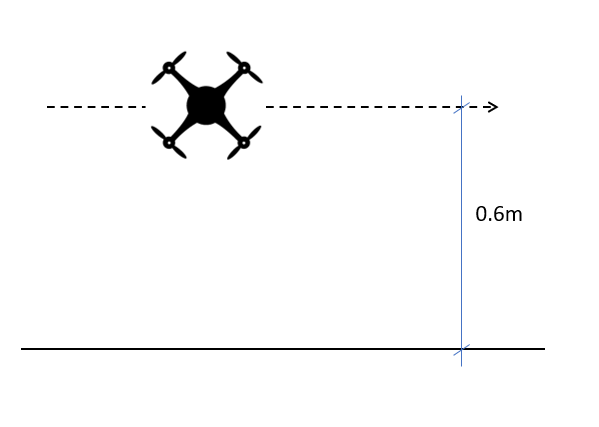
\includegraphics[width=0.30\textwidth]{modules/uneven_a}
    }
    \quad
    \subfloat[Stepped ground\label{fig:uneven_b}]{
        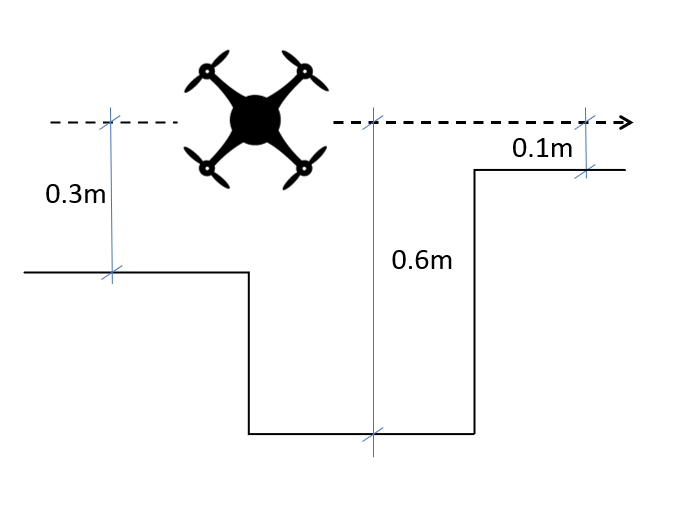
\includegraphics[width=0.30\textwidth]{modules/uneven_b}
    }
    \quad
    \subfloat[State estimator perspective of stepped ground\label{fig:uneven_c}]{
        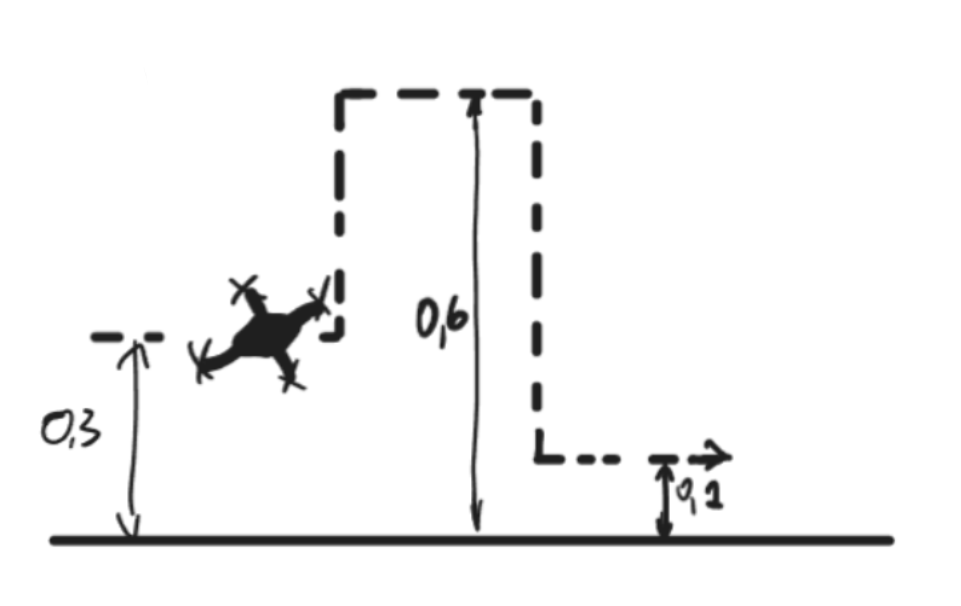
\includegraphics[width=0.30\textwidth]{modules/uneven_c}
    }
    \caption{Uneven floor problem.}\label{fig:uneven_floor}
\end{figure}

In the first Figure~\ref{fig:uneven_a}, the drone is flying over a flat ground, so the height sensor will contribute to the state estimate with the sensed value of 0.6 meters, which helps the State Estimator to provide a better estimate of the state (at least for the variable related with the height of the drone).

In the second Figure~\ref{fig:uneven_b}, the drone flies over a stepped ground. 
The height sensor will provide the State Estimator with a variable height by moving over this surface. 
The measured height will be either 0.6 or 0.1 meters, depending on the position.

Since the State Estimator is not aware of the conformation of the ground, the information perceived is the same as if the ground was flat and the drone was rapidly changing its height, as shown in Figure~\ref{fig:uneven_c}. 
The rapid change in the state estimate is not expected and can produce some instabilities in the flight.

To better understand the phenomena, we run some experiments with the following settings:
We placed a Crazyflie 2.1 with a height sensor attached in front of a cube-shaped obstacle with a height of 0.5 meters. 
We then write a script to take off the drone at 0.7 meters altitude and proceed above the obstacle. 
After passing the obstacle, the drone was supposed to land. 

As expected, as soon as the drone flies over the obstacle, the height sensor deck passes from a measure of 0.7 meters to a measure of 0.2 meters. 
This (unwanted) rapid change always makes the drone crash. 

To bypass this problem, we added a parameter that turns the height sensor's contribution to the state estimate on or off.
This way, when the application's environment has flat ground, the developer can enable the contribution and better estimate the drone's height.
Conversely, when the ground is uneven, the developer can avoid the problem described above by simply disabling the contribution through the parameter. 

\section{Lighthouse Module}\label{sec:module_lighthouse}

The Lighthouse ECF Module is the ECF Module associated with the Lighthouse Deck. As described in Section~\ref{subsec:absolute_positioning_systems}, the Lighthouse deck is a part of the absolute positioning system Lighthouse.
The Lighthouse positioning system consists of two (or more) base stations emitting infrared light signals in a sweeping pattern. 
The Lighthouse deck picks up these signals, which is mounted on the Crazyflie 2.1 drone. 
The deck then uses the received signals to calculate its precise position and orientation in 3D space.

This Module does not have a meaningful state. All the information that would belong to its state is technical and not applicable to any application.
Given this, the Lighthouse ECF module is an exception in the standard ECF Module implementation: it neither handles nor maintains a State.

A natural question can be: if the Lighthouse ECF Module does not hold a state, why is it useful?
To answer this question, we need a little bit of background on the functioning of the Lighthouse positioning system:
The Lighthouse positioning system is the most accurate and efficient positioning system that the whole Crazyflie platform provides. 
The problem related to this positioning system is the complex configuration.

The computation of the position in 3D space by knowing only the sweep angles of IR beams is not so direct. 
Indeed, to work correctly, the Lighthouse system needs a very accurate configuration based on multiple measurements taken in the flight space.

In fact, before using the Lighthouse, we need to estimate the environment's geometry. 
The system's geometry estimates the position and orientation of the two Lighthouse Base Stations with respect to the origin of the absolute positioning system.
To perform this estimation, the developer needs to measure the Geometry in multiple points of the flight space, and then by averaging them, he can get the best possible estimate.
The more accurate the Geometry estimation, the more precise the positioning system.

To answer the previous question, the Lighthouse ECF module exists and is extremely useful to overcome this limitation while using this positioning system.
The Lighthouse ECF Module is an ECF Module without state; it comprises numerous utility functions that help configure the Lighthouse positioning system.

The Lighthouse ECF Modules provide three main utility functions, each of which corresponds to a geometry estimation process:
\begin{itemize}
    \item \textit{simple\_geometry\_estimation}
    \item \textit{multi\_bs\_geometry\_estimation}
    \item \textit{automatic\_geometry\_estimation}
\end{itemize}
The first estimation process, \textit{simple\_geometry\_estimation}, is a very primitive and quick approach to the Geometry estimation process. 
It consists of a single measurement in one position in the 3D space. 
When this utility function is called, the ECF Module asks Crazyflie 2.1 for a single estimation of the position and orientation of the Lighthouse Base Stations.
When this information is received, the Module sets the measurement point as the origin of the 3D coordinate system. 
After that, it uploads this configuration back to Crazyflie 2.1.

A problem related to this type of estimation is that the error in the estimate is non-constant in the flight space. 
This problem happens because we only have a single measure in the entire flight space. 
As evident from Figure~\ref{fig:lighthouse_error_1}, it increases proportionally to the distance from the origin.
In this case, the resulting position estimate in the 3D space around the origin would be accurate. 
Still, as far as we move from the origin, the error in the drone position estimate will increase, possibly resulting in instabilities or even crashes.
This estimation process is intended only for quick tests where the drone position does not deviate too much from the origin.

\begin{figure}[tb]
    \centering
    \subfloat[Error distribution in the flight space while using the \textit{simple\_geometry\_estimation}\label{fig:lighthouse_error_1}]{
        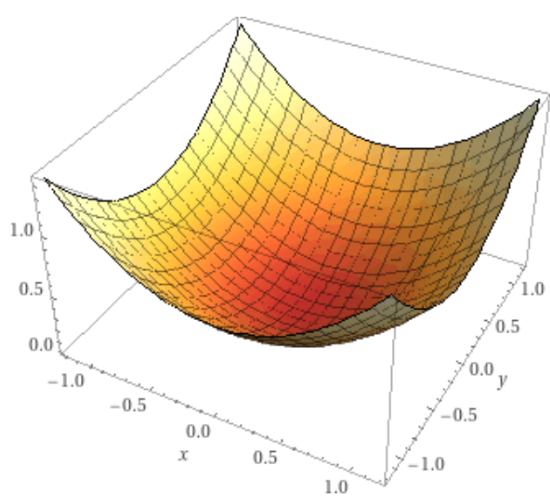
\includegraphics[width=0.40\textwidth]{modules/lighthouse_error_1}
    }
    \qquad
    \subfloat[ Error distribution in the flight space while using the \textit{multi\_bs\_geometry\_estimation}\label{fig:lighthouse_error_2}]{
        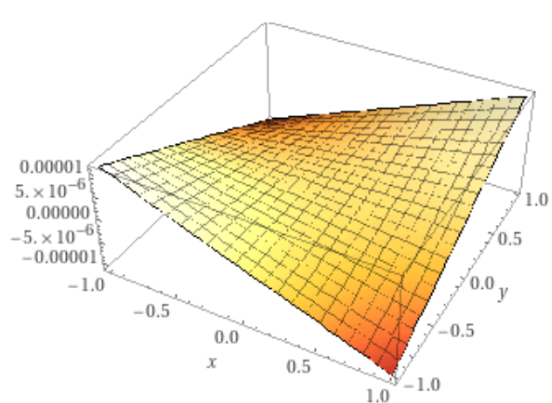
\includegraphics[width=0.40\textwidth]{modules/lighthouse_error_2}
    }
    \caption{Error distribution for Lighthouse.}\label{fig:lighthouse_error}
\end{figure}

To overcome this significant limitation, we developed a more accurate estimation process: \textit{multi\_bs\_geometry\_estimation}. 
As shown in Figure~\ref{fig:lighthouse_error_2}, this estimation process tries to make the error in the estimate constant across the entire flight space. 
Moreover, this estimation method also supports the presence of multiple Lighthouse Base Stations (more than 2) that significantly increase flight space.

This estimation method consists of multiple executions of the first estimation process.
All the recorded samples are averaged to build the most accurate geometry estimation sent to the Crazyflie 2.1.


The only drawback of this last estimation process is that it requires human help while doing the process. 
The problem is that the user moving the drone around the drone in the fourth phase is interfering with the estimation process. 
The user's body can block the IR beams from some base stations, invalidating lots of samples that otherwise would have been useful to compute a better geometry estimation.

The last estimation process, the \textit{automatic\_geometry\_estimation}, is the automation of the previous process. 
The user can configure the execution as he wants, and then the ECF Module (with the help of the Flow Deck v2) performs the sampling process by autonomously moving the drone around the flight space.

The \textit{automatic\_geometry\_estimation} is the most complex but most powerful estimation process.

\section{AI deck Module}\label{sec:module_ai_deck}


The AI Deck is an accessory board designed to provide on-board artificial intelligence (AI) capabilities to the Crazyflie 2.1, allowing it to perform advanced computational tasks without needing external processing.

The AI Deck is equipped with a powerful microcontroller unit (MCU) and a field-programmable gate array (FPGA), enabling high-performance computing and direct machine learning inference on the drone.
The MCU on the AI Deck can run complex algorithms and execute machine learning models. 
The FPGA complements the MCU by accelerating certain computations and enhancing the overall processing capabilities.

The AI Deck can communicate directly with the ground station via WiFi thanks to the NINA unit mounted on the deck.
The AI Deck, by default, runs a program on its MCU, which makes the video streaming of the camera mounted with the deck available on the WiFi communication channel.
For this work, we adopted this standard configuration of the AI Deck without implementing any algorithm for object tracking or anything similar.

The AI Deck ECF Module is an ECF module that allows one to connect, view, and run algorithms on the video streamed by the AI Deck itself.
When this ECF module is detected and created, it automatically tries to connect to the WiFi acces point held by the deck.

In particular, the Module consists of the following utility functions:
\begin{itemize}
    \item \textit{record}
    \item \textit{show\_recording}
    \item \textit{run\_ai}
\end{itemize}

The utility function \textit{record} allows the user to record from the video stream a video in mp4 format. 
This functionality is significant when the user is in the developing phase of an AI algorithm. 
In this case, the user can record videos and test/train their models using a flight recording.

The \textit{show\_recording} utility simply pops up a video player with the last unsaved recording, or if the path to the filename is provided, it shows the recording located at that path.

When the developer has completed its AI algorithm, the user can use the \textit{run\_ai} utility to run that algorithm on the real-time streaming from the camera and perform the actions needed to accomplish the goal of the application to be developed.

The \textit{run\_ai} function takes in input the algorithm (a python function) and an arbitrary list of arguments that can be used to take the actions.

This function looks very similar to a Subscription in our Coordination Manager with an Action (the algorithm) and a Context (the arguments) to an Observable that maintains the video stream.

Even if we could use our Coordination Framework, we decided to keep this particular implementation outside of it on purpose for two main reasons:
First, we did not want to overload the Coordination Framework with heavy data like images to make the complete state lighter.
Secondly, we thought that a direct implementation of the \textit{run\_ai} function would have been much easier to use in this case with respect to the standard subscription mechanism across the Coordination Framework.
